\documentclass[pdftex,12pt,a4paper]{report}
\usepackage[light,math]{iwona}
\usepackage[usenames,dvipsnames]{color}
\usepackage{tikz}
\usepackage{graphicx}
\newcommand{\HRule}{\rule{\linewidth}{0.5mm}}
\usetikzlibrary{datavisualization,calc,shapes,arrows,automata,trees,shadows,decorations.pathmorphing,positioning, shapes.misc,shapes.arrows,chains,matrix,scopes,decorations.pathmorphing,backgrounds}



\begin{document}
%
\begin{titlepage}
\begin{center}
% Upper part of the page


\textsc{\color{Sepia}{\LARGE EC~320}}\\[1.5cm]
\textsc{\Large Week~One}\\[0.5cm]
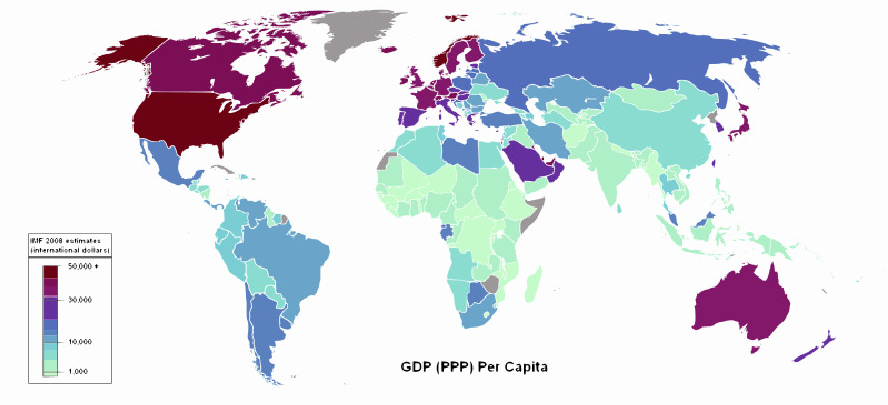
\includegraphics[scale=0.5]{GDP}\\
\cite{wiki:001}
% Title
\HRule \\[0.4cm]
{ \huge \bfseries Principles of Macroeconomics}\\[0.4cm]
\HRule \\[1.5cm]


% Author and supervisor
\begin{minipage}{0.4\textwidth}
\begin{flushleft} \large
\emph{Author:}\\
Jason \textsc{Mansfield}
\end{flushleft}
\end{minipage}
\begin{minipage}{0.4\textwidth}
\begin{flushright} \large
\emph{Instructor:} \\
Dr.~Anthony \textsc{Pizur}
\end{flushright}
\end{minipage}

\vfill

% Bottom of the page
{\large \today}


\end{center}
\end{titlepage}
As shown in \textbf{figure 1} the Opportunity cost when studying or teaching Science or Mathematics results in a loss of time which could have been spent enjoying the arts or other cultural practices. 
\begin{figure}[Production–possibility frontier]
\caption{Production~Possibility Frontier}
\begin{tikzpicture}
 \draw [->] (-1,0) -- (10,0);
\draw [->] (0,-1) -- (0,10);
\draw [dashed] (0, 5) -- (6,5) -- (6,0);
\draw [dashed] (0, 7) -- (4.4,7) -- (4.4,0);
\draw [x=10ex,y=10ex](5,0) sin (0,5);
\draw (1.1,5.2) node {\color{blue}{Mathmatics}};
\draw (5.9,0.2) node {\color{red}{Cultural Exploration}};
\draw (1.1,7.2) node {\color{Sepia}{Science}};
\draw (4.1,0.9) node {\color{orange}{Art}};
\end{tikzpicture}
\end{figure}
\clearpage
% bib stuff
    \nocite{*}
    \bibliographystyle{apalike}
    \bibliography{cite}

\end{document}